\Exercise[label={ex:NLO2},title={coses}] 
A company wants to maximize its profit function given by:

\[
f(x, y) = -x^2 + 4xy - 2y^2
\]

where \(x\) and \(y\) represent the amount of resources allocated to two different projects.

The problem is subject to the following constraints:
\begin{enumerate}
    \item The total resources used must not exceed 30 units:
    \[
    x + 2y \leq 30
    \]
    \item The product of the resources allocated must be at least 50 units:
    \[
    xy \geq 50
    \]
    \item The relationship between the resource allocations must satisfy the following nonlinear constraint:
    \[
    y \leq \frac{3x^2}{100} + 5
    \]
\end{enumerate}

The company wants to find the values of \(x\) and \(y\) that maximize the profit \(f(x, y)\) under these constraints. 

Can you help the company drawing the problem in a graph? Can you identify the feasible region? Is the region convex?


\Answer 

This is \autoref{ex:NLO2}.

A company wants to maximize its profit function given by:

\[
f(x, y) = -x^2 + 4xy - 2y^2
\]

where \(x\) and \(y\) represent the amount of resources allocated to two different projects.

The problem is subject to the following constraints:
\begin{enumerate}
    \item The total resources used must not exceed 30 units:
    \[
    x + 2y \leq 30
    \]
    \item The product of the resources allocated must be at least 50 units:
    \[
    xy \geq 50
    \]
    \item The relationship between the resource allocations must satisfy the following nonlinear constraint:
    \[
    y \leq \frac{3x^2}{100} + 5
    \]
\end{enumerate}


Find the values of \(x\) and \(y\) that maximize the profit \(f(x, y)\) under these constraints.


The problem is shown in Figure \ref{Fig:NLO2}.

\begin{minipage}[t]{\linewidth}
  \vspace{-2ex}
        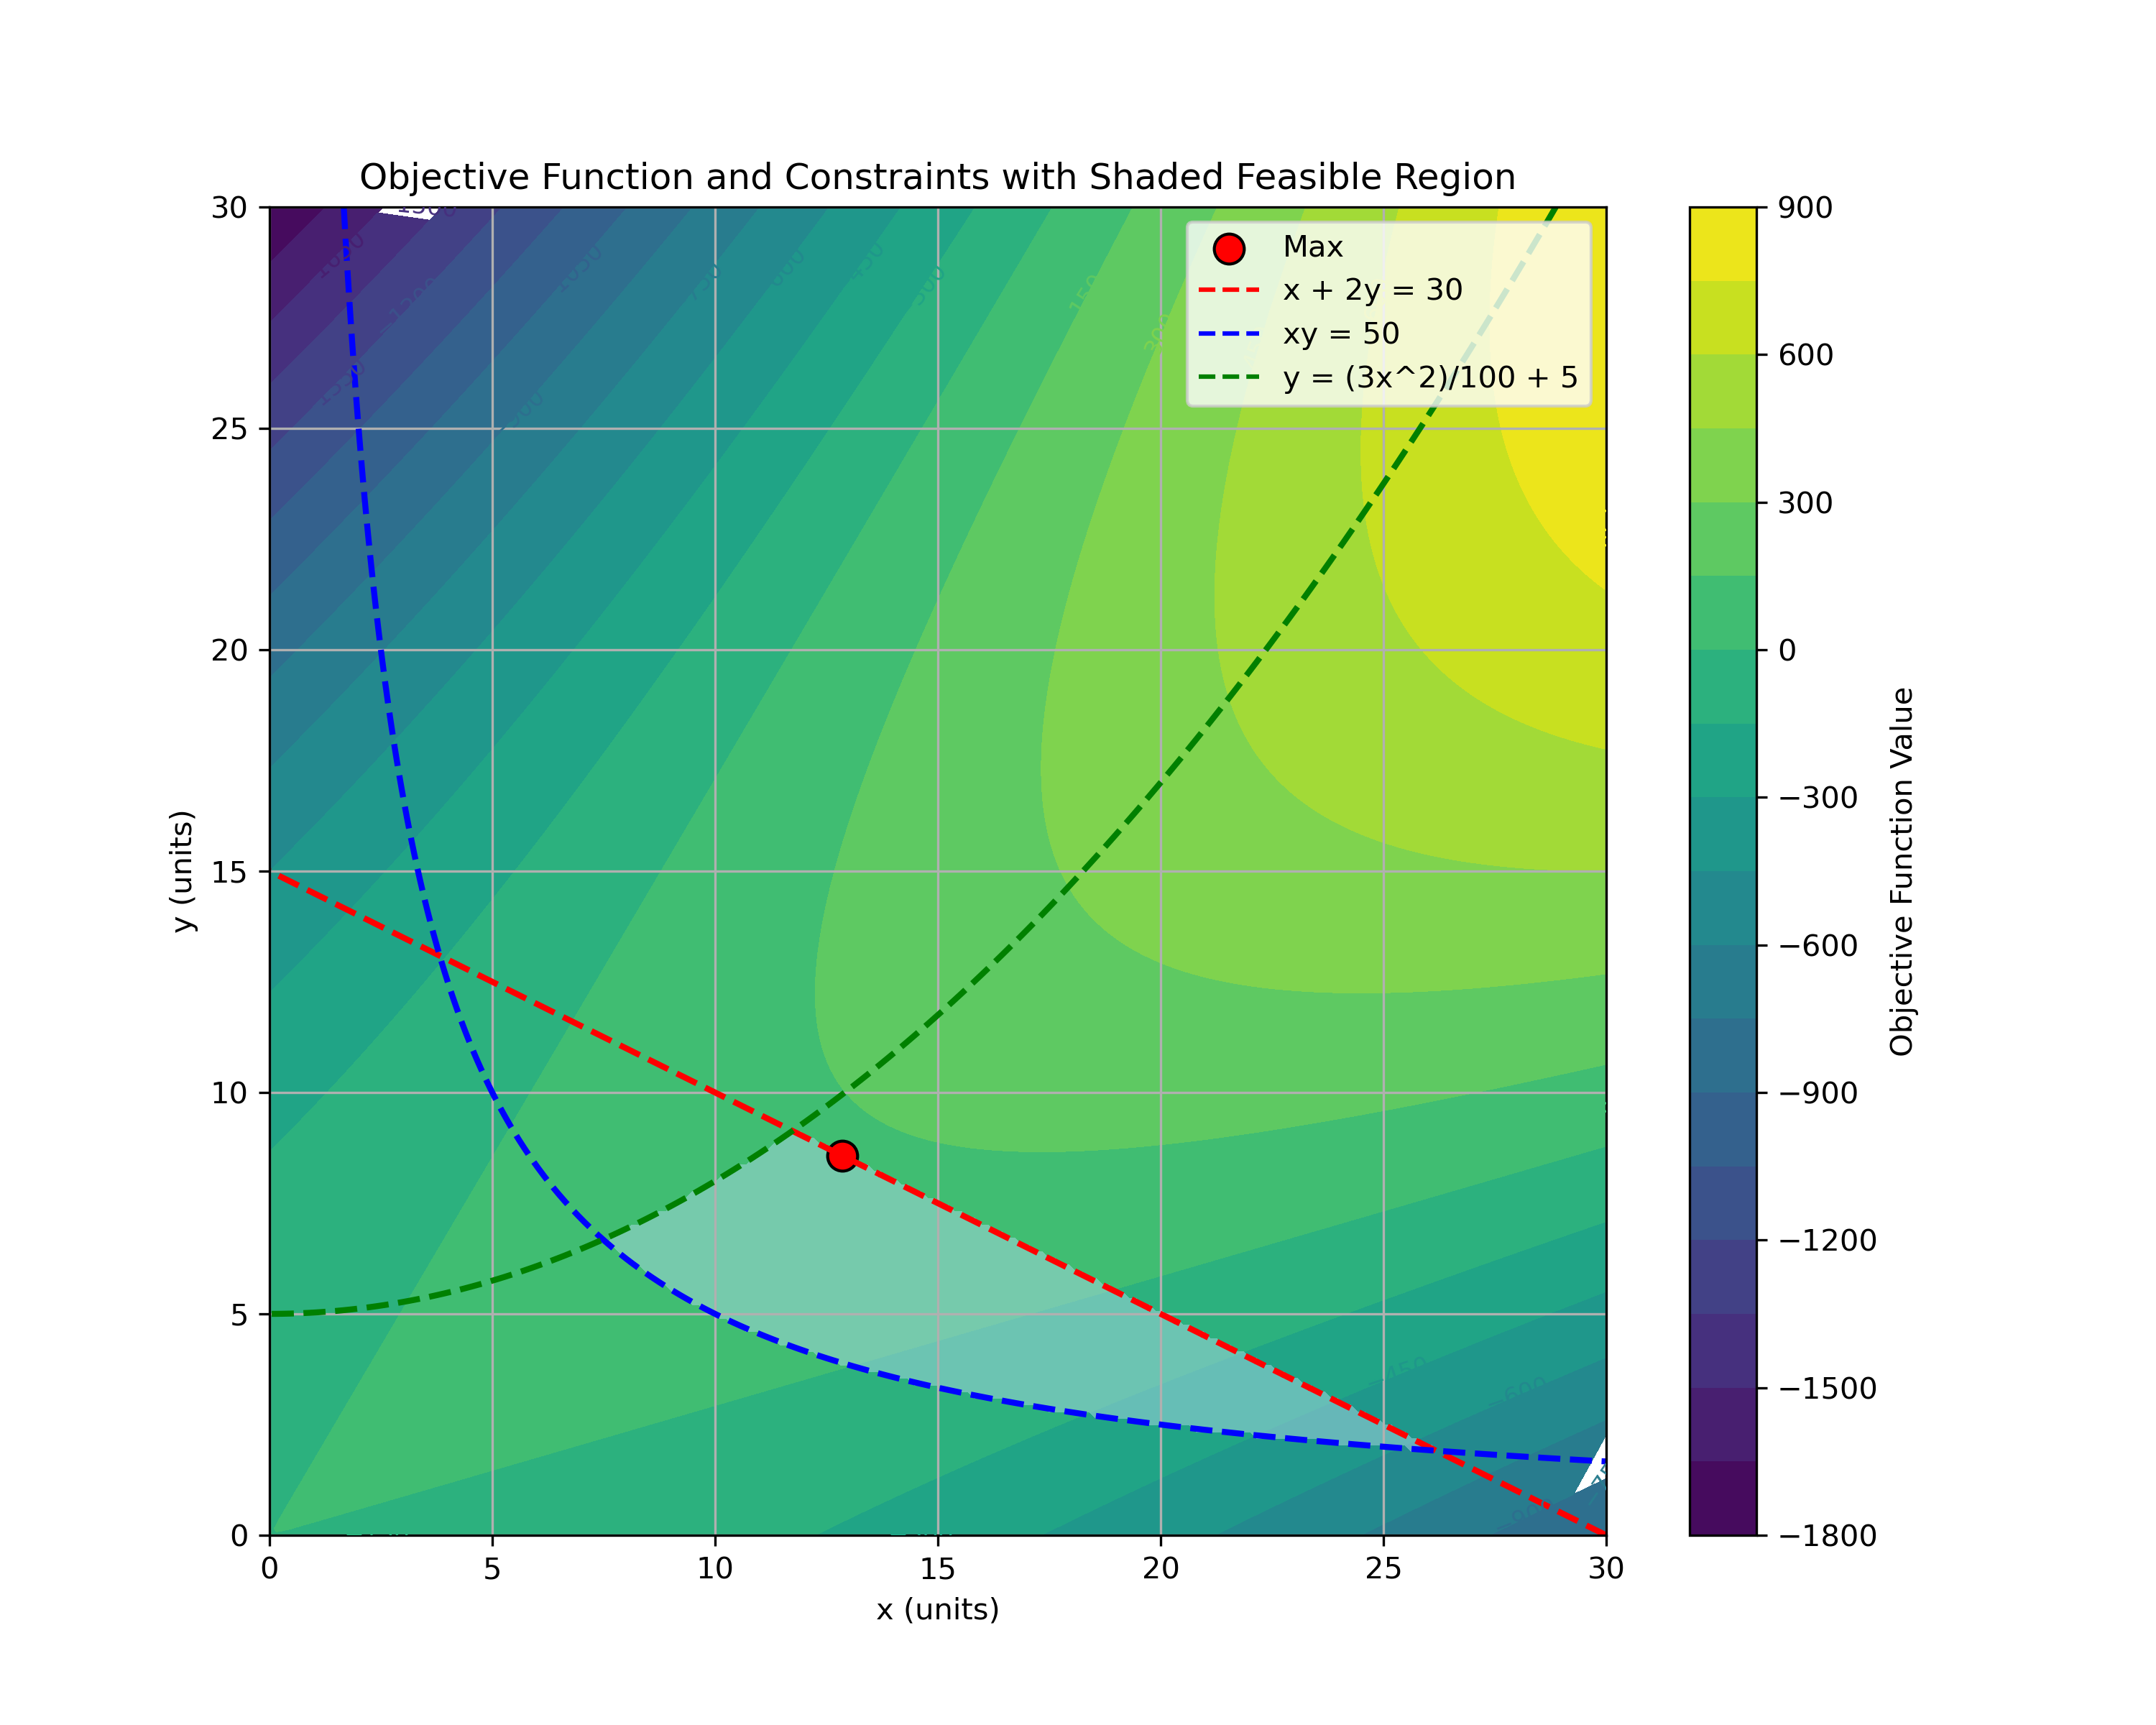
\includegraphics[scale=0.7]{NLO2.png}
        \captionof{figure}{Contour plot of the objective function \( f(x, y) = -x^2 + 4xy - 2y^2 \) with constraints \(x + 2y \leq 30\) (red dashed), \(xy \geq 50\) (blue dashed), and \(y \leq \frac{3x^2}{100} + 5\) (green dashed). The light blue region represents the feasible area where all constraints are satisfied. The solution obtained with \autoref{code:NLO2}}
    \label{Fig:NLO2}
\end{minipage}

\blacksquare